% Twelve Views of Thai Tourism -- manuscript
% Build: python -m src.build_paper   (pdflatex -> bibtex -> pdflatex x2)
\documentclass{article}

% ---------------------------------------------------------------- layout
\usepackage{preprint}   % arXiv-style preprint layout, see paper/preprint.sty
\usepackage{microtype}

% ---------------------------------------------------------------- packages
\usepackage{amsmath}
\usepackage{graphicx}
\graphicspath{{../figures/}}
\usepackage{booktabs,tabularx,array}
\usepackage[table]{xcolor}
\usepackage[font=small,labelfont=bf,labelsep=period,justification=justified,singlelinecheck=false,skip=6pt]{caption}
\usepackage{enumitem}
\setlist{itemsep=2pt,topsep=4pt}
\usepackage{tikz}
\usetikzlibrary{positioning}
\usepackage[authoryear,round]{natbib}
\setlength{\bibsep}{2pt}
\usepackage[section]{placeins}
\usepackage[colorlinks=true,linkcolor=blue!45!black,citecolor=blue!45!black,urlcolor=blue!45!black]{hyperref}
\hypersetup{pdftitle={Twelve Views of Thai Tourism}, pdfauthor={Thanatchon Chongmankhong}}
\renewcommand{\topfraction}{0.9}
\renewcommand{\bottomfraction}{0.8}
\renewcommand{\textfraction}{0.08}
\renewcommand{\floatpagefraction}{0.75}

% Generated by src/analysis.py -- do not edit by hand
\newcommand{\FirstYear}{2010}
\newcommand{\FirstM}{16.6}
\newcommand{\PeakYear}{2019}
\newcommand{\PeakM}{39.7}
\newcommand{\LowYear}{2021}
\newcommand{\LowM}{0.39}
\newcommand{\LatestYear}{2025}
\newcommand{\LatestM}{32.4}
\newcommand{\RecoveryPct}{81.6}
\newcommand{\DropPct}{99.0}
\newcommand{\CagrPct}{10.2}
\newcommand{\SeasonPeakMonth}{December}
\newcommand{\SeasonPeak}{1.23}
\newcommand{\SeasonLowMonth}{May}
\newcommand{\SeasonLow}{0.81}
\newcommand{\SeasonRatio}{1.52}
\newcommand{\TopPre}{China}
\newcommand{\TopPreShare}{27.7}
\newcommand{\TopLatest}{China}
\newcommand{\TopLatestShare}{14.4}
\newcommand{\HhiPre}{1,273}
\newcommand{\HhiLatest}{943}
\newcommand{\UnitsTopRegion}{ASEAN}
\newcommand{\UnitsTop}{33}
\newcommand{\UnitsAsia}{69}
\newcommand{\StayShort}{Malaysia}
\newcommand{\StayShortN}{3}
\newcommand{\StayLong}{Germany}
\newcommand{\StayLongN}{16}
\newcommand{\StayRatio}{5.3}
\newcommand{\FirstBkkPct}{38.9}
\newcommand{\StyleBeachPct}{31.0}
\newcommand{\StyleCityPct}{38.2}
\newcommand{\EuAndamanPct}{29.8}
\newcommand{\AseanBorderPct}{44.3}
\newcommand{\OnwardTotalM}{18.3}
\newcommand{\OnwardBkkPct}{81.4}
\newcommand{\OnwardTopFrom}{Bangkok}
\newcommand{\OnwardTopTo}{Pattaya \& East}
\newcommand{\OnwardTopM}{2.68}
\newcommand{\PattayaBkkM}{1.87}
\newcommand{\NetNodes}{35}
\newcommand{\NetEdges}{76}
\newcommand{\NetBkkEdges}{29}
\newcommand{\NetSameRegionPct}{49.1}
\newcommand{\NetBkkDegreePct}{25.9}
\newcommand{\NetTopA}{Phuket}
\newcommand{\NetTopB}{Krabi}
\newcommand{\NetTopK}{870}
\newcommand{\RevTotalBn}{2,127}
\newcommand{\RevTopOne}{Bangkok}
\newcommand{\RevTopOnePct}{35.2}
\newcommand{\RevTopFivePct}{84.1}
\newcommand{\RevHhi}{2,087}
\newcommand{\RevGini}{0.92}
\newcommand{\SpendHi}{Phuket}
\newcommand{\SpendHiV}{51,650}
\newcommand{\SpendLo}{Sa Kaeo}
\newcommand{\SpendLoV}{2,700}
\newcommand{\SpendRatio}{19}
\newcommand{\SpendRho}{0.49}
\newcommand{\SpendCatOne}{Accommodation}
\newcommand{\SpendCatOnePct}{28.5}
\newcommand{\SpendCatTwo}{Shopping}
\newcommand{\SpendCatTwoPct}{24.0}
\newcommand{\SpendCatThree}{Food \& drink}
\newcommand{\SpendCatThreePct}{21.0}
\newcommand{\SpendTopThreePct}{73.5}
\newcommand{\SpendTopLeaf}{Three- and four-star hotels}
\newcommand{\SpendTopLeafPct}{12.5}
\newcommand{\ProfN}{15}
\newcommand{\ProfR}{0.06}
\newcommand{\ProfSpendHi}{Singapore}
\newcommand{\ProfSpendHiV}{6,500}
\newcommand{\ProfSpendLo}{Laos}
\newcommand{\ProfSpendLoV}{3,000}
\newcommand{\ProfRepeatHi}{Laos}
\newcommand{\ProfRepeatHiPct}{82}
\newcommand{\SegN}{1,200}
\newcommand{\SegK}{6}
\newcommand{\SegSilEmbed}{0.48}
\newcommand{\SegSilFeat}{0.23}
\newcommand{\SegAri}{0.85}
\newcommand{\SegLargest}{City shoppers}
\newcommand{\SegLargestPct}{22.8}
\newcommand{\RecSeasonR}{0.998}
\newcommand{\RecSeasonMae}{0.006}
\newcommand{\RecDropPlanted}{99.0}
\newcommand{\RecDropObs}{99.0}
\newcommand{\RecStayMae}{0.32}
\newcommand{\RecStayMax}{0.5}
\newcommand{\RecDestMae}{0.37}
\newcommand{\RecDestMax}{1.77}
\newcommand{\RecHubPlanted}{81.8}
\newcommand{\RecHubObs}{81.4}

\newcommand{\inputrows}[1]{\csname @@input\endcsname #1 }  % primitive \input works inside tabular

\definecolor{rqa}{HTML}{2A78D6}
\definecolor{rqb}{HTML}{17A2A2}
\definecolor{rqc}{HTML}{C2414B}
\definecolor{rqd}{HTML}{8E5BB5}

\title{Twelve Views of Thai Tourism: A Data-Shape-Driven Framework for Visual Analysis,
Evaluated by Planted-Structure Recovery}
\author{Thanatchon Chongmankhong\\
  {[Affiliation]}\\
  \texttt{[email]}}
\date{November 2026}
\renewcommand{\shorttitle}{Twelve Views of Thai Tourism}

\begin{document}
\maketitle

\begin{abstract}
Tourism data are rarely of a single shape. A single research programme may require seasonal time
series, origin--destination flows, hierarchical expenditure accounts, co-visitation networks and
multivariate traveller profiles, yet empirical reporting in tourism continues to rely predominantly on bar and
line charts. We propose a data-shape-driven framework that derives visual idioms from research questions
through an explicit abstraction of the data, and instantiate it as twelve coordinated views organised around
four questions: who visits and when, where visitors go, where the money goes, and what kinds of travellers
there are. To evaluate the framework independently of the availability and quality of administrative data,
we design a simulation study following the ADEMP structure, in which known structure---seasonality, a
pandemic shock, the diversification of source markets, destination preferences, a hub-and-spoke pattern of
onward travel, revenue concentration and six latent traveller personas---is planted in ten synthetic
datasets spanning \FirstYear--\LatestYear. Each view is paired with a companion statistic, and recovery of
the planted structure is measured. The views recover the seasonal profile ($r = \RecSeasonR$), median
length of stay (mean absolute error \RecStayMae{} nights), destination preferences (\RecDestMae{}
percentage points) and persona membership (adjusted Rand index \SegAri), while making visible features
that tabular summaries obscure, including the near-total collapse of arrivals in \LowYear{} and a double
concentration of revenue in a handful of provinces. An open, single-command pipeline regenerates every
number, table and figure. All results derive from synthetic data and illustrate the method; they are not
empirical findings about Thai tourism.
\end{abstract}

\keywords{Visual analytics \and Data visualisation \and Tourism analytics \and Simulation study \and
  Synthetic data \and Reproducible research}

% ================================================================
\section{Introduction}\label{sec:intro}

Tourism is among the most data-rich sectors of the Thai economy. Statistical agencies publish monthly
arrivals by nationality; expenditure surveys disaggregate visitor spending by category; and passively
collected mobility, card-payment and booking data increasingly trace where visitors travel within the
country. These sources differ not only in provenance and quality but in \emph{shape}. A monthly arrivals
series is a cyclical time series; the movement of visitors from source markets to destinations is a
multi-stage flow; an expenditure account is a hierarchy; co-visitation between provinces is a network; and a
visitor survey is a high-dimensional table of individuals. A research programme on inbound tourism will
typically encounter all of these shapes at once.

Visual reporting has not kept pace with this heterogeneity. Policy reports and empirical studies continue to
rely predominantly on bar, line and pie charts---idioms designed for low-dimensional tables. When cyclical
series, multi-stage flows or hierarchies are compressed into such charts, the structure of analytical
interest---periodicity, pathways, concentration, latent groups---becomes difficult to perceive and must
instead be recovered from tables or narrative. The visualisation literature offers a mature repertoire of
idioms matched to particular data abstractions \citep{heer2010zoo,munzner2014}, but two gaps remain. First,
there is little guidance on how such idioms should be \emph{composed} within a single, domain-specific
research programme, so that each view answers a distinct question and the views together cover the problem.
Second, claims that a given idiom ``reveals'' a structure are seldom tested against known ground truth; in
empirical work the true structure is, by definition, unknown.

This paper addresses both gaps. We propose a data-shape-driven framework that derives visual idioms from
research questions through an explicit abstraction of the data, and we instantiate it as twelve coordinated
views organised around four research questions for inbound tourism:
\begin{description}[leftmargin=3.2em,labelwidth=2.6em,itemsep=1pt]
  \item[RQ1] Who visits, and when?
  \item[RQ2] Where do visitors go, and how do they move between destinations?
  \item[RQ3] Where does tourism revenue accrue, and on what is it spent?
  \item[RQ4] What kinds of travellers are there, and how do they differ?
\end{description}
To evaluate the framework independently of the availability and quality of administrative data, we embed
it in a simulation study \citep{morris2019}. Known structure is planted in ten synthetic datasets; each view
is paired with a companion statistic; and the accuracy with which the planted structure is recovered is
measured.

The paper makes four contributions:
\begin{enumerate}[label=(C\arabic*),leftmargin=3em]
  \item A framework that maps four tourism research questions to twelve visual idioms through explicit data
        abstractions, together with five design principles shared by all views (Section~\ref{sec:framework}).
  \item A planted-structure evaluation protocol, organised by the ADEMP structure for simulation studies, which
        pairs each idiom with a companion statistic and quantifies recovery of known structure
        (Sections~\ref{sec:study} and~\ref{sec:results}).
  \item An open, reproducible implementation in which every number, table and figure in this paper is
        regenerated from source by a single command (Section~\ref{sec:implementation}).
  \item Practical guidance on the trade-off between expressiveness and perceptual accuracy, and on replacing
        the synthetic inputs with official data (Section~\ref{sec:discussion}).
\end{enumerate}

We use synthetic data deliberately. Doing so separates the evaluation of the method from questions of data
access and quality and, crucially, supplies the ground truth against which recovery can be measured. The
corollary is that none of the numerical results reported here are empirical findings about Thai tourism;
they show what the framework reveals when the structure is known. Section~\ref{sec:related} reviews related
work, Section~\ref{sec:framework} presents the framework, Section~\ref{sec:study} describes the simulation
study, Section~\ref{sec:results} reports the results, Section~\ref{sec:discussion} discusses implications,
threats to validity and limitations, and Section~\ref{sec:conclusion} concludes.

% ================================================================
\section{Background and related work}\label{sec:related}

\subsection{From data abstraction to visual idiom}
Contemporary visualisation theory frames design as a mapping from a data abstraction and a task abstraction
to a visual encoding \citep{munzner2014}. Perceptual experiments establish a ranking of encoding channels:
position along a common scale is judged more accurately than length, angle, area or colour saturation
\citep{cleveland1984}. The ranking bears directly on idioms that rely on angle, such as sunbursts and chord
diagrams, or on area, such as circle packing, and it motivates the fifth of our design principles.
\citet{heer2010zoo} catalogue idioms by the shape of the data---time series, statistical distributions,
maps, hierarchies and networks---which is the organising idea of the present framework. \citet{segel2010}
show that ordering multiple views into a narrative sequence helps readers to follow an argument, which informs
the sequencing of views within each research question.

\subsection{Flows, networks and hierarchies}
Sankey diagrams encode flow magnitude as band width and suit multi-stage flows \citep{riehmann2005}. Chord
diagrams, popularised by Circos \citep{krzywinski2009}, arrange groups around a circle and show flows
between pairs in both directions, which makes asymmetry visible. Dense networks quickly become illegible in
node--link form; hierarchical edge bundling \citep{holten2006} routes edges along a hierarchy so that they
aggregate into bundles, trading the legibility of individual edges for the visibility of group-level
structure. For hierarchies, sunbursts encode proportion as angle on concentric rings \citep{stasko2000},
whereas circle packing encodes size as area within nested circles \citep{wang2006}, sacrificing space
efficiency for clearly delineated groups. Unit charts descend from Neurath's Isotype \citep{neurath1936}, in
which one symbol represents a fixed quantity; they communicate proportions to audiences with little
training in reading charts.

\subsection{Temporal and distributional views}
ThemeRiver \citep{havre2000} and streamgraphs \citep{byron2008} depict changing composition as a continuous
flow; \citet{byron2008} derive the ``wiggle'' baseline that minimises the slope of the layers. For periodic
data, spiral layouts \citep{weber2001} align equivalent phases of successive cycles and so expose recurrent
patterns that a long linear series obscures. Ridgeline plots stack partially overlapping distributions to
compare their shapes across groups \citep{wilke2019}, and beeswarm plots extend the dot plot
\citep{wilkinson1999} by displacing points to avoid overlap, so that every unit remains visible.

\subsection{Multivariate structure}
Parallel coordinates \citep{inselberg1985} map each variable to a vertical axis and each item to a polyline,
revealing correlation and clusters as bundles of lines. Non-linear dimensionality reduction methods such as
t-SNE \citep{vandermaaten2008} and UMAP \citep{mcinnes2018} project high-dimensional data into two dimensions
while preserving local neighbourhoods. Their output is easily over-interpreted: cluster sizes and distances
between clusters in a t-SNE map are not, in general, meaningful \citep{wattenberg2016}. We therefore pair the
embedding with an independent clustering in the original feature space.

\subsection{Visualisation in tourism research}
Tourism research has long-standing conceptual frameworks with temporal and spatial content, notably the
tourism area life cycle \citep{butler1980}, and the COVID-19 pandemic prompted extensive assessment of the
sector's exposure to shocks \citep{gossling2021}. The visual presentation of such analyses nonetheless relies
largely on basic charts. Our contribution is not a new idiom but a principled way of selecting and composing
existing idioms so that, together, they cover the questions a tourism research programme asks.

\subsection{Simulation studies and planted structure}
Simulation studies are the standard means of evaluating statistical methods when ground truth is required.
\citet{morris2019} propose the ADEMP structure---aims, data-generating mechanisms, estimands, methods and
performance measures---for their design and reporting. Visualisation research more often relies on user
studies or case studies. We adapt ADEMP to visual analysis by treating each planted structure as an estimand
and each view, paired with a companion statistic, as a method whose ability to recover the estimand can be
quantified.

% ================================================================
\section{A data-shape-driven framework}\label{sec:framework}

\subsection{From questions to data shapes}
The framework proceeds in three steps (Figure~\ref{fig:framework}). First, a research question is stated in
domain terms. Second, the data required to answer it are abstracted into a shape: a composition, a cyclical
or compositional time series, a set of distributions, a multi-stage or pairwise flow, a hierarchy, a network
or a multivariate table. Third, an idiom is chosen whose encoding matches that shape, preferring the most
accurate channel that can still express the structure of interest. Table~\ref{tab:framework} lists the
resulting twelve pairings with the principal encoding and the feature a reader should look for. Cartographic
views are excluded deliberately: choropleth and flow maps are well established in tourism reporting, and the
purpose here is to examine idioms that remain under-used.

\begin{figure}[!htbp]
\centering
\begin{tikzpicture}[
  font=\sffamily\footnotesize,
  rq/.style={rounded corners=2pt, fill=#1, text=white, minimum height=14mm, text width=33mm, align=center, inner sep=3pt},
  tq/.style={rounded corners=2pt, draw=#1, fill=#1!7, minimum height=9.5mm, text width=33mm, align=center, inner sep=2.5pt},
  node distance=2mm]
\node[rq=rqa] (A) at (0,0)     {\textbf{RQ1}\\Who visits,\\and when?};
\node[rq=rqb] (B) at (3.85,0)  {\textbf{RQ2}\\Where do\\visitors go?};
\node[rq=rqc] (C) at (7.7,0)   {\textbf{RQ3}\\Where does\\the money go?};
\node[rq=rqd] (D) at (11.55,0) {\textbf{RQ4}\\What kinds\\of travellers?};
\node[tq=rqa, below=of A]  (A1) {\textbf{Unit chart}\\composition};
\node[tq=rqa, below=of A1] (A2) {\textbf{Radial spiral}\\cyclical time series};
\node[tq=rqa, below=of A2] (A3) {\textbf{Streamgraph}\\composition over time};
\node[tq=rqa, below=of A3] (A4) {\textbf{Ridgeline plot}\\distributions by group};
\node[tq=rqb, below=of B]  (B1) {\textbf{Sankey diagram}\\multi-stage flow};
\node[tq=rqb, below=of B1] (B2) {\textbf{Chord diagram}\\pairwise flow};
\node[tq=rqb, below=of B2] (B3) {\textbf{Edge bundling}\\network in a hierarchy};
\node[tq=rqc, below=of C]  (C1) {\textbf{Circle packing}\\hierarchy with size};
\node[tq=rqc, below=of C1] (C2) {\textbf{Sunburst}\\hierarchy with proportion};
\node[tq=rqc, below=of C2] (C3) {\textbf{Beeswarm}\\all units on one axis};
\node[tq=rqd, below=of D]  (D1) {\textbf{Parallel coordinates}\\multivariate profiles};
\node[tq=rqd, below=of D1] (D2) {\textbf{Embedding map}\\similarity in many dimensions};
\node[draw=black!35, fill=black!4, rounded corners=2pt, text width=148mm, align=center, minimum height=8mm,
      below=5mm of A4.south west, anchor=north west]
  {Ten synthetic datasets $\rightarrow$ companion statistics $\rightarrow$ twelve figures $\rightarrow$ manuscript,
   regenerated by one command (\texttt{python run\_all.py})};
\end{tikzpicture}
\caption{The framework. Four research questions (top row) are mapped to twelve idioms through the shape of the
data each question requires (boxes below). All views are produced by a single reproducible pipeline (bottom).}
\label{fig:framework}
\end{figure}

\begin{table}[!htbp]
\centering
\caption{Research questions, data shapes and idioms.}
\label{tab:framework}
\small
\renewcommand{\arraystretch}{1.1}
\begin{tabularx}{\linewidth}{@{}l>{\raggedright\arraybackslash}p{2.9cm}>{\raggedright\arraybackslash}p{2.75cm}>{\raggedright\arraybackslash}X>{\raggedright\arraybackslash}X@{}}
\toprule
RQ & Data shape & Idiom & Principal encoding & Look for \\
\midrule
RQ1 & Composition & Unit chart & One square per visitor; colour by region & Dominant origin regions \\
    & Cyclical time series & Radial spiral & Angle = month; radius = arrivals; colour = year & Recurrent seasonality; contraction and recovery \\
    & Composition over time & Streamgraph & Layer thickness = arrivals & Growing and shrinking markets \\
    & Distributions by group & Ridgeline plot & Height = share of trips & Centre and spread of stays \\
\midrule
RQ2 & Multi-stage flow & Sankey diagram & Band width = travellers & Market-specific pathways \\
    & Pairwise flow & Chord diagram & Ribbon-end width = directional flow & Hubs and asymmetry \\
    & Network in a hierarchy & Edge bundling & Edges routed through the hierarchy; width = trips & Regional circuits and bridges \\
\midrule
RQ3 & Hierarchy with size & Circle packing & Area = revenue & Concentration of revenue \\
    & Hierarchy with proportion & Sunburst & Angle = share of spending & Dominant categories and items \\
    & All units on one axis & Beeswarm & Position = spend per visitor; area = visitors & Inequality between provinces \\
\midrule
RQ4 & Multivariate profiles & Parallel coordinates & Position on parallel axes & Co-moving markets and trade-offs \\
    & Similarity in many dimensions & Embedding map & Proximity = similarity & Traveller segments and overlaps \\
\bottomrule
\end{tabularx}
\end{table}

\subsection{Design principles}
Five principles apply to every view.
\begin{description}[leftmargin=2.2em,labelwidth=1.8em,itemsep=2pt]
  \item[D1] \emph{One view, one question.} Each view is assigned to exactly one research question, and its
        caption states what the reader should see before describing how it is encoded.
  \item[D2] \emph{Colour follows identity, not rank.} Each family of categories---origin regions, Thai regions,
        destination clusters, spending categories and personas---has its own palette, and a category keeps its
        colour wherever it appears.
  \item[D3] \emph{Stable order.} Categories appear in the same order in every view.
  \item[D4] \emph{Direct labelling.} Labels sit on the marks wherever space permits; legends are used only where
        direct labels would occlude data.
  \item[D5] \emph{Pair angle and area with numbers.} Views that rely on angle or area, channels judged less
        accurately than position \citep{cleveland1984}, are accompanied by printed values or a companion table.
\end{description}

% ================================================================
\section{Simulation study design}\label{sec:study}

We report the study following the ADEMP structure \citep{morris2019}.

\subsection{Aims}
The study has two aims: (i) to demonstrate that each of the twelve views answers its research question on data
of realistic shape; and (ii) to quantify, for every view whose structure has a ground-truth parameter, how
accurately the view's companion statistic recovers the planted structure.

\subsection{Data-generating mechanisms}\label{sec:dgm}
All ten datasets (Table~\ref{tab:datasets}) are generated from a single seed (2026), with an independent random
stream for each dataset, so that every table is reproducible exactly. The mechanisms are deliberately simple
and transparent; their parameters are listed in Appendix~\ref{app:params}.

\paragraph{Arrivals by market}
For each of ten named markets $k$ and year $t \in \{2010,\dots,2025\}$, arrivals follow a prescribed
trajectory $a_{kt}$ with small multiplicative noise,
\begin{equation}
A_{kt} = a_{kt}\,(1 + \varepsilon_{kt}), \qquad \varepsilon_{kt} \sim \mathcal{N}(0, 0.004^2).
\end{equation}
For seven residual groups $g$, pre-pandemic arrivals interpolate linearly between prescribed 2010 and 2019
levels with $\mathcal{N}(0, 0.02^2)$ noise and a 5\% dip in 2014. From 2020 onwards,
$A_{gt} = \pi_t A_{g,2019}(1+\varepsilon_{gt})$, with pandemic multipliers
$\pi = (0.17, 0.02, 0.33, 0.74, 0.92, 0.93)$ for 2020--2025.

\paragraph{Monthly arrivals}
Annual totals $A_t = \sum_k A_{kt}$ are allocated to months by
\begin{equation}
A_{tm} = \lfloor A_t\, w_{tm} \rfloor, \qquad
w_{tm} = \frac{\omega_{tm}(1+\eta_{tm})}{\sum_{m'} \omega_{tm'}(1+\eta_{tm'})}, \qquad
\eta_{tm} \sim \mathcal{N}(0, 0.025^2),
\end{equation}
with the rounding residual added to December so that months sum exactly to the annual total. The profile
$\omega_{tm}$ equals a common seasonal profile $\omega_m$ in ordinary years, with year-specific profiles for
2014 (a mid-year dip), 2020--2023 (pandemic collapse and recovery) and 2025.

\paragraph{Length of stay}
Nights per trip for market $k$ follow a log-normal distribution with median $\mu_k$ and log-scale
$\sigma_k$, discretised to $\{1,\dots,30\}$ and renormalised.

\paragraph{Trip flows}
For origin region $o$ with latest-year arrivals $T_o$, destination shares are
$p_{d\mid o} \propto P_{od}(1+\xi_{od})$ with $\xi_{od} \sim \mathcal{N}(0, 0.04^2)$, and trip-style shares
are $q_{s\mid d,o} \propto Q_{ds}\,\tau_{os}$, where $\tau$ tilts the style mix by origin. Flows are
$F_{ods} = T_o\, p_{d\mid o}\, q_{s\mid d,o}$, rounded to the nearest hundred.

\paragraph{Onward travel, provinces and co-visits}
Onward trips between six destination clusters scale a prescribed matrix $R$ by
$(1+\mathcal{N}(0, 0.05^2))$. For the 77 provinces, 44 have prescribed visitor volumes and spend per
visitor; the remainder draw volumes from $\mathcal{U}(15, 90)$ thousand and spend from
$\mathcal{U}(2{,}800, 8{,}500)$ THB. Revenue is the product of visitors and spend. Co-visitation among 35
provinces is defined by 76 plausible pairs with multiplicative $\mathcal{N}(0, 0.05^2)$ noise.

\paragraph{Spending structure}
A fixed three-level hierarchy with 21 leaves allocates shares of total visitor spending to categories,
sub-categories and items.

\paragraph{Traveller personas}
A survey of $n = \SegN$ respondents is drawn from a mixture of six personas $z$ with prior weights
$\pi_z$. Each respondent has eight features: log spend per day, nights, age, group size and four activity
intensities (beach, shopping, culture and nightlife). Features equal persona means plus noise (log spend,
$\sigma = 0.32$; log nights, $\sigma = 0.42$; age, $\sigma = 9$ years; group size, $\sigma = 1.0$;
activities, $\sigma = 0.2$, clipped to $[0,1]$); the origin region is drawn from a persona-specific
categorical distribution.

\begin{table}[!htbp]
\centering
\caption{The ten synthetic datasets.}
\label{tab:datasets}
\small
\begin{tabularx}{\linewidth}{@{}l>{\raggedright\arraybackslash}Xrr@{}}
\toprule
Dataset & Content & Rows & Columns \\
\midrule
\inputrows{generated/tab_datasets.tex}
\bottomrule
\end{tabularx}
\end{table}

\subsection{Estimands}
The planted structures, or estimands, are: (E1) the seasonal profile of twelve monthly indices; (E2) the depth
of the pandemic shock, measured as the proportional fall in arrivals from 2019 to 2021; (E3) the
diversification of source markets between 2019 and \LatestYear; (E4) the median length of stay in nine
markets; (E5) destination preferences $p_{d\mid o}$, comprising 36 shares; (E6) the hub share of onward
travel, defined as the share of onward trips that involve Bangkok; (E7) the concentration of revenue across
provinces; and (E8) the membership of \SegN{} respondents in six personas. For E1, E2, E4, E5, E6 and E8 the
data-generating mechanism defines a ground-truth value. E3 and E7 are emergent properties of prescribed
inputs, for which we report observed values only.

\subsection{Methods}
Each view is paired with a companion statistic that summarises what the view shows. The seasonal index of
month $m$ is the mean ratio of that month to its year's monthly mean over the pre-pandemic years
$Y = \{2010, \dots, 2019\}$,
\begin{equation}
S_m = \frac{1}{|Y|} \sum_{y \in Y} \frac{A_{ym}}{\bar{A}_y}.
\end{equation}
Concentration is measured by the Herfindahl--Hirschman index and the Gini coefficient,
\begin{equation}
\mathrm{HHI} = \sum_{i=1}^{n} (100\, s_i)^2, \qquad
G = \frac{\sum_{i=1}^{n} (2i - n - 1)\, x_{(i)}}{n \sum_{i=1}^{n} x_i},
\end{equation}
where $s_i$ is the share of unit $i$ and $x_{(i)}$ are the values in ascending order; HHI ranges from 0 to
10{,}000. Monotone association is measured by Spearman's $\rho$. For personas, respondents are embedded with
t-SNE (perplexity 40, PCA initialisation); separation is summarised by the silhouette coefficient
\citep{rousseeuw1987} in the embedding and in feature space; and $k$-means ($k = 6$, 20 initialisations) on the
standardised features is compared with true membership by the adjusted Rand index (ARI) \citep{hubert1985}.

\subsection{Performance measures}
For the profile estimand E1 we report Pearson's $r$ and the mean absolute error (MAE) between recovered and
planted values. For E4 and E5 we report the MAE and the maximum absolute error in natural units (nights and
percentage points). For the scalar estimands E2 and E6 we report planted and recovered values, and for E8 the
ARI.

\subsection{Implementation and reproducibility}\label{sec:implementation}
The pipeline is written in Python using NumPy, pandas, SciPy, scikit-learn \citep{pedregosa2011} and
Matplotlib \citep{hunter2007}. Every figure is drawn directly in Matplotlib. Idioms absent from standard
libraries were implemented for this study: a chord layout following the algorithm of D3 \citep{bostock2011},
hierarchical edge bundling with cubic B-splines and bundling strength $\beta$ \citep{holten2006}, and a
variable-radius beeswarm placement. Circle packing uses the \texttt{circlify} library. Smoothed curves in the
streamgraph and ridgeline plot use monotone piecewise cubic interpolation \citep{fritsch1980}, which passes
through every data point without overshoot. The analysis script writes every reported number as a \LaTeX{}
macro and every table body as a file, so that the manuscript is regenerated from the data; a test suite
checks internal consistency, for example that monthly arrivals sum to annual totals. The complete pipeline
runs in about a minute on a laptop.

% ================================================================
\section{Results}\label{sec:results}

\subsection{RQ1: who visits, and when?}

\begin{figure}[!htbp]
\centering
\begin{minipage}[t]{0.42\linewidth}
  \centering
  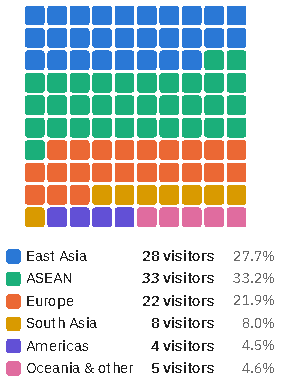
\includegraphics[width=\linewidth]{fig02_unit_chart}
  \caption{Unit chart. International arrivals in \LatestYear{} reduced to one hundred visitors; one square per
  visitor, coloured by origin region and apportioned by largest remainder.}
  \label{fig:unit}
\end{minipage}\hfill
\begin{minipage}[t]{0.54\linewidth}
  \centering
  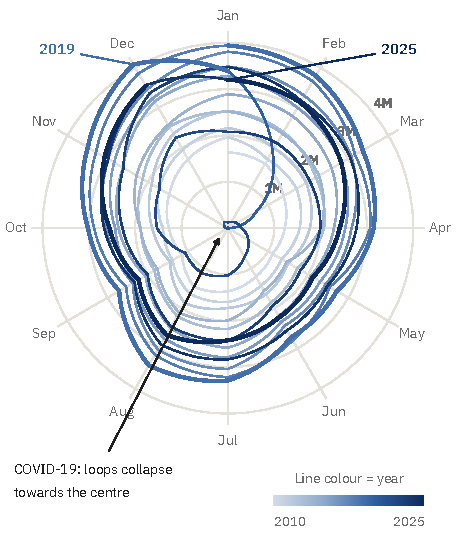
\includegraphics[width=\linewidth]{fig03_radial_spiral}
  \caption{Radial spiral. Monthly arrivals, \FirstYear--\LatestYear; one revolution per year, radius
  proportional to arrivals. Thick lines mark the peak and the latest year.}
  \label{fig:spiral}
\end{minipage}
\end{figure}

Figure~\ref{fig:unit} reduces the latest year's arrivals to one hundred visitors. In the synthetic data,
\UnitsTopRegion{} is the largest origin region (\UnitsTop{} of 100), and the three Asian regions together
account for \UnitsAsia{} of every 100 visitors. The unit chart conveys composition at a glance, which makes it
a suitable opening view for non-specialist audiences.

Figure~\ref{fig:spiral} shows monthly arrivals on a radial spiral. Successive loops expand during the
pre-pandemic period, with compound annual growth of \CagrPct\%, until the peak year, \PeakYear{}
(\PeakM{} million). They then collapse towards the centre in \LowYear{} (\LowM{} million, a fall of
\DropPct\%) before expanding again to \RecoveryPct\% of the peak in \LatestYear. The shape of each loop
conveys seasonality: the seasonal index peaks in \SeasonPeakMonth{} (\SeasonPeak) and reaches its minimum in
\SeasonLowMonth{} (\SeasonLow), a ratio of \SeasonRatio. On a linear time axis the same 192 observations
make the recurrent annual pattern considerably harder to discern.

\begin{figure}[!htbp]
\centering
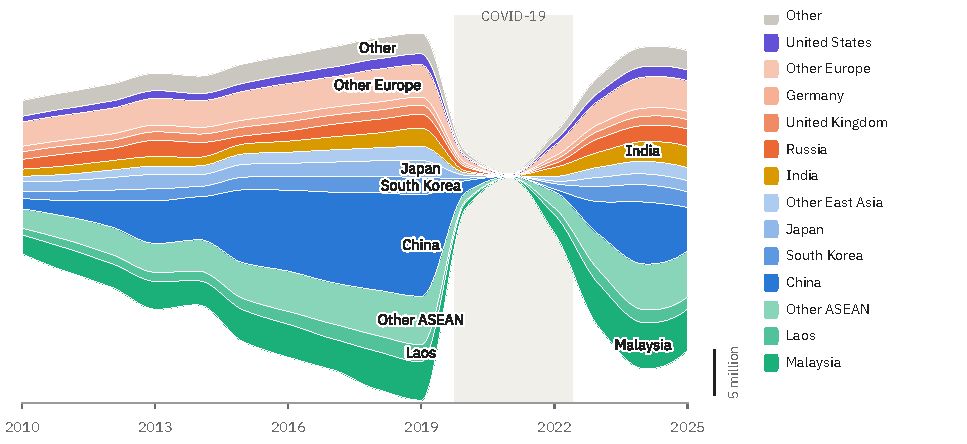
\includegraphics[width=\linewidth]{fig04_streamgraph}
\caption{Streamgraph. Annual arrivals by market; layer thickness is proportional to arrivals, drawn on the
wiggle baseline of \citet{byron2008}. Markets from the same origin region share a colour family; the grey band
marks the pandemic. Curves are smoothed by monotone cubic interpolation for display.}
\label{fig:stream}
\end{figure}

Figure~\ref{fig:stream} shows how the composition of source markets changed. The largest single market
(\TopPre) accounted for \TopPreShare\% of arrivals in 2019 but \TopLatestShare\% in \LatestYear, while ASEAN
and South Asian markets recovered faster. The HHI of source markets accordingly fell from \HhiPre{} to
\HhiLatest, indicating a more diversified market base. The change is visible directly in the thickness of the
layers, without pairwise comparison of annual bar charts.

\begin{figure}[!htbp]
\centering
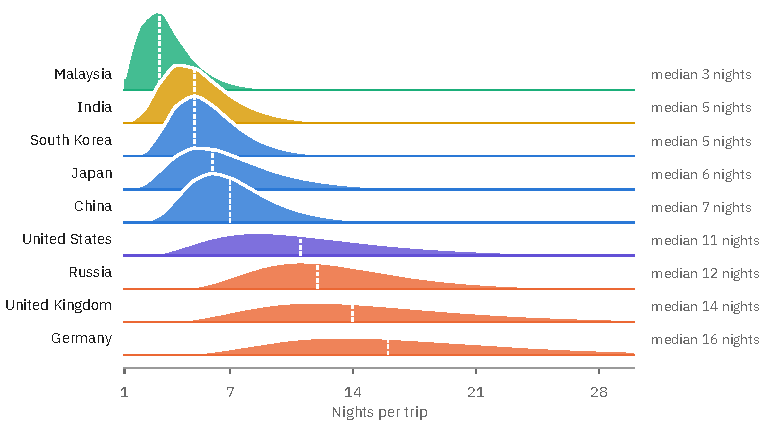
\includegraphics[width=\linewidth]{fig05_ridgeline}
\caption{Ridgeline plot. Distribution of nights per trip by market, ordered by median; dashed white lines mark
medians, colours follow origin region.}
\label{fig:ridge}
\end{figure}

Figure~\ref{fig:ridge} shows that the length of stay differs markedly by market. The median ranges from
\StayShortN{} nights (\StayShort) to \StayLongN{} nights (\StayLong), a \StayRatio-fold difference. Beyond
central tendency, the shapes of the distributions are informative: short-haul markets have narrow,
right-skewed distributions, whereas European markets have broad distributions with long tails. A single mean
per market would conceal the difference.

\FloatBarrier
\subsection{RQ2: where do visitors go?}

\begin{figure}[!htbp]
\centering
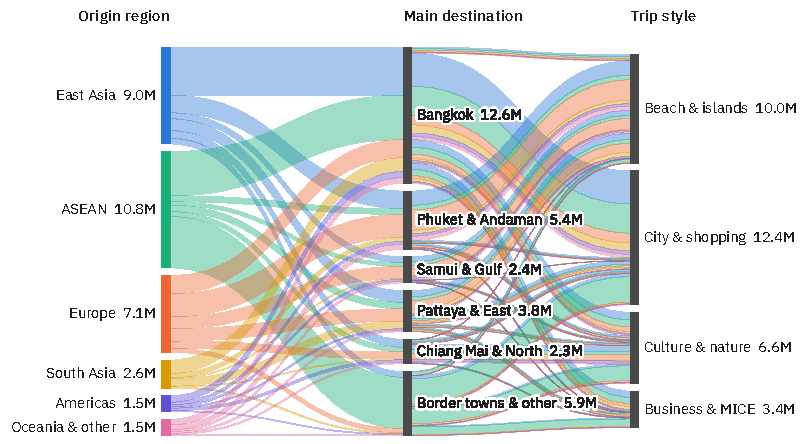
\includegraphics[width=\linewidth]{fig06_sankey}
\caption{Three-stage Sankey diagram: origin region, main destination and trip style, \LatestYear. Band width
is proportional to travellers. Second-stage bands are split by origin, so that each region's colour runs
through the whole diagram.}
\label{fig:sankey}
\end{figure}

Figure~\ref{fig:sankey} traces each origin region through its main destination to its trip style. Bangkok is
the main destination for \FirstBkkPct\% of visitors; city-and-shopping trips account for \StyleCityPct\% and
beach-and-island trips for \StyleBeachPct\%. Because second-stage bands are split by origin, colours run
continuously through the diagram and expose market-specific pathways: \EuAndamanPct\% of European visitors head
primarily for the Andaman coast, and \AseanBorderPct\% of ASEAN visitors for border towns. The same information
in a three-way cross-tabulation is close to illegible.

\begin{figure}[!htbp]
\centering
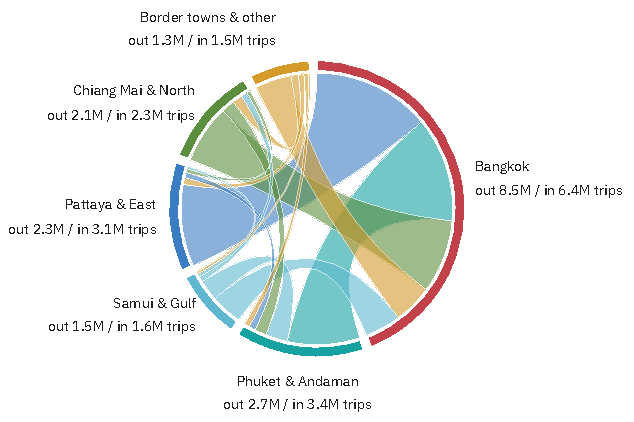
\includegraphics[width=0.92\linewidth]{fig07_chord}
\caption{Chord diagram of onward trips between six destination clusters. The width of each end of a ribbon is
proportional to the flow in that direction; arc length is proportional to outgoing trips. Ribbons take the
colour of the smaller cluster in each pair.}
\label{fig:chord}
\end{figure}

Figure~\ref{fig:chord} examines movement between destination clusters. Onward trips total \OnwardTotalM{}
million, and Bangkok is involved in \OnwardBkkPct\% of them. The largest flow runs from \OnwardTopFrom{} to
\OnwardTopTo{} (\OnwardTopM{} million), and the diagram makes its asymmetry visible: the reverse flow is only
\PattayaBkkM{} million. The difference in width between the two ends of a single ribbon is the chord diagram's
distinctive advantage over a matrix of numbers.

\begin{figure}[!htbp]
\centering
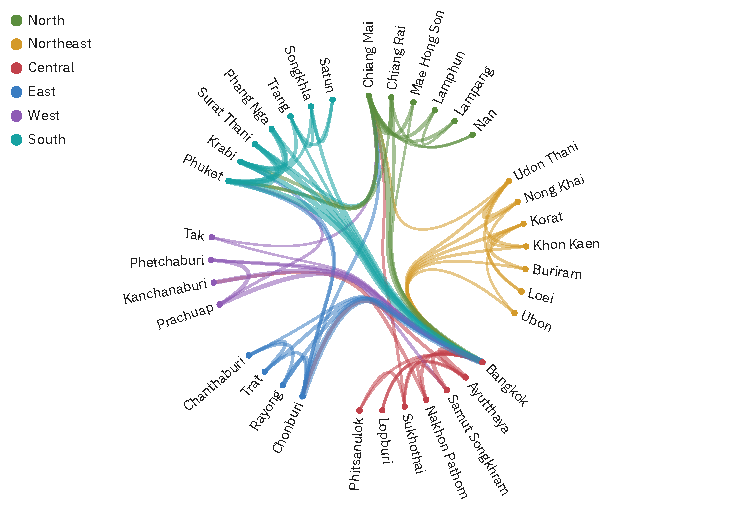
\includegraphics[width=\linewidth]{fig08_edge_bundling}
\caption{Hierarchical edge bundling of provinces visited on the same trip. Provinces are arranged by region;
edges are cubic B-splines routed through regional control points and the root ($\beta = 0.85$), with width
proportional to trips and colour taken from the less-connected province of each pair.}
\label{fig:bundle}
\end{figure}

Figure~\ref{fig:bundle} descends to the level of provinces. The co-visitation network has \NetNodes{}
provinces and \NetEdges{} pairs; Bangkok participates in \NetBkkEdges{} pairs and accounts for
\NetBkkDegreePct\% of the total weighted degree. Yet \NetSameRegionPct\% of the network's weight lies within
regions---in the Andaman triangle and the northern circuit, for example---and the strongest pair not involving
Bangkok is \NetTopA--\NetTopB{} (\NetTopK{} thousand trips). Read together, the three views of RQ2 operate at
three scales: the market, the destination cluster and the province.

\FloatBarrier
\subsection{RQ3: where does the money go?}

\begin{figure}[!htbp]
\centering
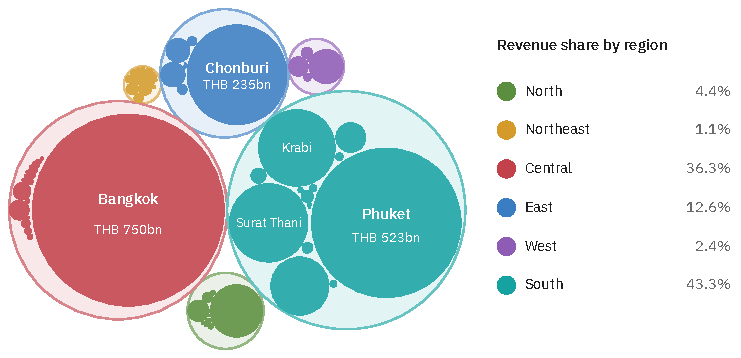
\includegraphics[width=\linewidth]{fig09_circle_packing}
\caption{Circle packing of revenue from foreign visitors by province, grouped by region; circle area is
proportional to revenue.}
\label{fig:pack}
\end{figure}

\begin{table}[!htbp]
\centering
\caption{The eight provinces with the highest revenue from foreign visitors.}
\label{tab:provinces}
\small
\begin{tabular}{@{}llrrrr@{}}
\toprule
Province & Region & Visitors (m) & Spend per visitor (THB) & Revenue (THB bn) & Share (\%) \\
\midrule
\inputrows{generated/tab_provinces.tex}
\bottomrule
\end{tabular}
\end{table}

Revenue across all provinces totals THB \RevTotalBn{} billion. Figure~\ref{fig:pack} and
Table~\ref{tab:provinces} show extreme concentration: \RevTopOne{} alone accounts for \RevTopOnePct\% and the
five leading provinces for \RevTopFivePct\%; the Gini coefficient is \RevGini{} and the HHI \RevHhi. The packed
circles convey the inequality immediately, but comparisons of area are coarse, hence the companion table
(principle D5).

\begin{figure}[!htbp]
\centering
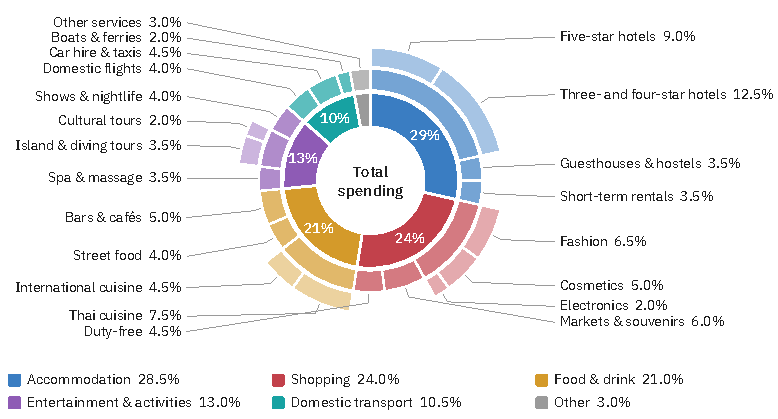
\includegraphics[width=\linewidth]{fig10_sunburst}
\caption{Sunburst of visitor spending: categories (inner ring), sub-categories (middle) and items (outer); angle
is proportional to the share of total spending.}
\label{fig:sunburst}
\end{figure}

Figure~\ref{fig:sunburst} shows that three categories---\SpendCatOne{} (\SpendCatOnePct\%), \SpendCatTwo{}
(\SpendCatTwoPct\%) and \SpendCatThree{} (\SpendCatThreePct\%)---account for \SpendTopThreePct\% of spending.
The outer rings reveal structure hidden within categories: the largest single item is
\SpendTopLeaf{} (\SpendTopLeafPct\%), so that accommodation spending is concentrated in the mid-to-upper
segment of the hotel market---information relevant to the design of policies that aim to distribute tourism
income more widely.

\begin{figure}[!htbp]
\centering
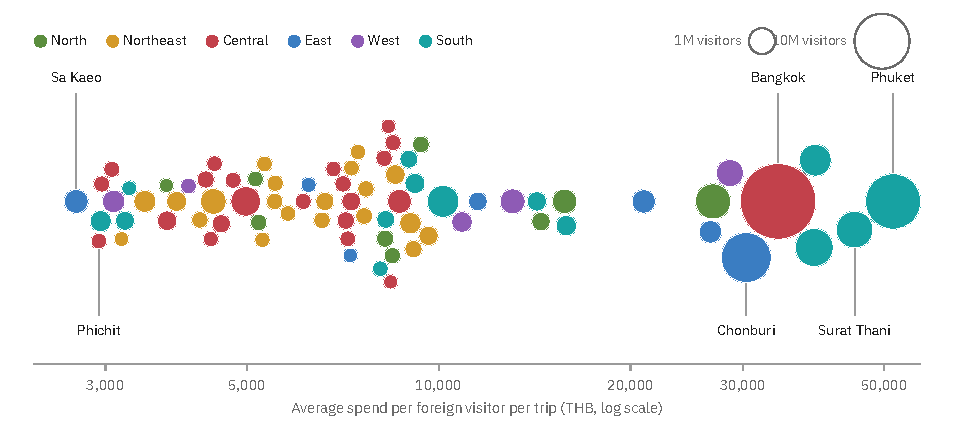
\includegraphics[width=\linewidth]{fig11_beeswarm}
\caption{Beeswarm of the 77 provinces. Horizontal position is the average spend per foreign visitor per trip
(log scale); circle area is proportional to the number of foreign visitors; colour denotes region.}
\label{fig:swarm}
\end{figure}

Figure~\ref{fig:swarm} places every province on a single axis. Spend per visitor ranges from THB \SpendLoV{}
(\SpendLo) to THB \SpendHiV{} (\SpendHi), a factor of about \SpendRatio. Border provinces that receive short
visits from neighbouring countries cluster on the left, coastal resort provinces on the right. The Spearman
correlation between visitor volume and spend per visitor is \SpendRho: provinces that attract more visitors
also earn more from each visitor, so that concentration operates at two levels at once.

\FloatBarrier
\subsection{RQ4: what kinds of travellers are there?}

\begin{figure}[!htbp]
\centering
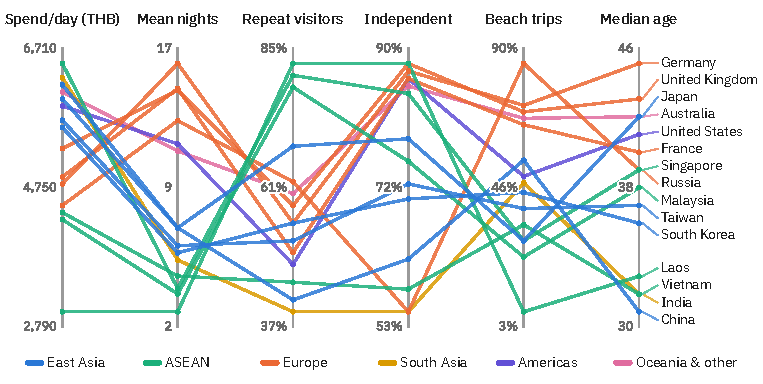
\includegraphics[width=\linewidth]{fig12_parallel_coordinates}
\caption{Parallel coordinates of \ProfN{} market profiles on six variables. Each axis is scaled to its own
range; colours follow origin region.}
\label{fig:parallel}
\end{figure}

Figure~\ref{fig:parallel} compares \ProfN{} markets on six variables simultaneously. \ProfSpendHi{} has the
highest spend per day (THB \ProfSpendHiV), \ProfSpendLo{} the lowest (THB \ProfSpendLoV), and
\ProfRepeatHi{} also has the highest share of repeat visitors (\ProfRepeatHiPct\%). Across markets, the
correlation between nights per trip and spend per day is only $r = \ProfR$: in these data, longer stays do not
imply lower daily spending. Crossing polylines make such trade-offs visible in a way a table does not; European
markets, for instance, sit high on nights and on the share of beach trips but mid-range or low on daily spend.

\begin{figure}[!htbp]
\centering
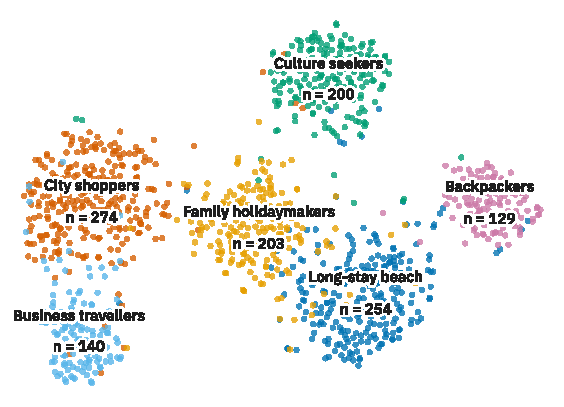
\includegraphics[width=0.74\linewidth]{fig13_embedding}
\caption{Embedding map. t-SNE projection of \SegN{} synthetic survey respondents from eight features,
coloured by the persona used to generate them. Distances between clusters should not be interpreted literally.}
\label{fig:embed}
\end{figure}

\begin{table}[!htbp]
\centering
\caption{Median profiles of the six traveller segments.}
\label{tab:segments}
\small
\begin{tabular}{@{}lrrrrrl@{}}
\toprule
Segment & $n$ & Share (\%) & Spend/day (THB) & Nights & Age & Most common origin \\
\midrule
\inputrows{generated/tab_segments.tex}
\bottomrule
\end{tabular}
\end{table}

Figure~\ref{fig:embed} projects the \SegN{} respondents into two dimensions; Table~\ref{tab:segments} gives
the median profile of each segment. The largest segment is \SegLargest{} (\SegLargestPct\%). The silhouette
coefficient is \SegSilEmbed{} in the embedding but only \SegSilFeat{} in the original feature space, a
reminder that t-SNE accentuates separation \citep{wattenberg2016}. $k$-means clustering in the original space
nevertheless recovers the personas with an ARI of \SegAri, which confirms that the clusters exist in the data
rather than being an artefact of the projection.

\FloatBarrier
\subsection{Recovery of planted structure}

\begin{table}[!htbp]
\centering
\caption{Recovery of planted structure. MAE: mean absolute error; pp: percentage points; ARI: adjusted Rand index.}
\label{tab:recovery}
\small
\renewcommand{\arraystretch}{1.1}
\begin{tabularx}{\linewidth}{@{}l>{\raggedright\arraybackslash}X>{\raggedright\arraybackslash}p{3.3cm}>{\raggedright\arraybackslash}p{4.6cm}@{}}
\toprule
 & Estimand & View & Recovery \\
\midrule
\inputrows{generated/tab_recovery.tex}
\bottomrule
\end{tabularx}
\end{table}

Table~\ref{tab:recovery} summarises recovery. The seasonal index reproduces the planted profile almost exactly
($r = \RecSeasonR$, MAE $= \RecSeasonMae$), and the recovered depth of the pandemic shock (\RecDropObs\%) matches
its noise-free planted value (\RecDropPlanted\%). Median lengths of stay are recovered with an MAE of
\RecStayMae{} nights, the residual being entirely attributable to the discretisation of stays to whole nights.
Destination preferences read from the Sankey diagram deviate from the planted shares by \RecDestMae{}
percentage points on average, reflecting the noise injected into the flow mechanism. The hub share of onward
travel is recovered as \RecHubObs\% against a planted \RecHubPlanted\%, and persona membership with an ARI of
\SegAri. In every case the residual error is attributable to a known source---injected noise, discretisation
or rounding---rather than to the view itself. Recovery here is, however, statistical: it establishes that the
information needed to see each structure is present in what the view encodes, not that readers will perceive
it (Section~\ref{sec:validity}).

% ================================================================
\section{Discussion}\label{sec:discussion}

\subsection{Complementary views across scales}
The framework does not prescribe that all twelve views be used in every study. It shows, rather, that a single
research question frequently requires more than one scale of analysis. RQ2 is the clearest case: the Sankey
diagram answers where each market goes, the chord diagram which destinations feed one another, and edge
bundling which provinces are visited together. Each reveals structure that the other two cannot. Likewise, RQ3
requires size (circle packing), proportion (sunburst) and distribution (beeswarm) to distinguish inequality
that arises from visitor volumes from inequality that arises from spending per visitor.

\subsection{Expressiveness and perceptual accuracy}
Elaborate idioms repay their cost when the shape of the data matches the shape of the view---a cycle and a
spiral, a flow and a band---but they trade away accuracy in reading individual values. Angles in sunbursts and
areas in circle packing are judged less accurately than positions \citep{cleveland1984}; distances in a t-SNE
map are not distances in the data \citep{wattenberg2016}; and parallel coordinates become hard to read beyond a
few dozen items. The practical implication is to use expressive views to reveal patterns and to confirm the
values that matter with tables or position-based charts (principle D5), and to sequence views as a narrative
that follows the research questions \citep{segel2010} rather than presenting them all at once.

\subsection{From synthetic to empirical data}
The pipeline is designed so that real data with the same columns can replace the synthetic inputs without
changes to the plotting code. Table~\ref{tab:realdata} lists the kinds of sources that could substitute for
each dataset. Flows and co-visitation are typically the hardest to obtain because they require individual-level
mobility data, which must be aggregated before use to protect privacy.

\begin{table}[!htbp]
\centering
\caption{Candidate empirical sources for each synthetic dataset.}
\label{tab:realdata}
\small
\begin{tabularx}{\linewidth}{@{}>{\raggedright\arraybackslash}p{4.5cm}>{\raggedright\arraybackslash}X>{\raggedright\arraybackslash}p{4.4cm}@{}}
\toprule
Synthetic dataset & Candidate source & Caveats \\
\midrule
\texttt{arrivals\_by\_nationality}, \texttt{arrivals\_monthly} & Official monthly statistics of international
arrivals by nationality & Definitions of arrivals versus tourists differ \\
\texttt{stay\_length}, \texttt{nationality\_profiles}, \texttt{spending\_breakdown} & Surveys of visitor behaviour
and expenditure & Sampling weights and survey error must be reported \\
\texttt{trip\_flows}, \texttt{region\_flows}, \texttt{province\_covisits} & Mobile positioning, card-payment or
booking data & Privacy; aggregation required before use \\
\texttt{provinces} & Provincial statistics on visitors and tourism receipts & Definitions of revenue vary by
source \\
\texttt{traveler\_segments} & Individual-level visitor surveys & Ethical review required \\
\bottomrule
\end{tabularx}
\end{table}

\subsection{Threats to validity}\label{sec:validity}
\emph{Construct validity.} Recovery is measured on companion statistics, not on human readers. That a view
encodes the information required to see a structure does not establish that readers perceive it, perceive it
quickly or perceive it correctly; establishing this requires controlled user studies.
\emph{Internal validity.} The planted structures were designed by the author, which creates a risk of
designing data that flatter the views. Noise is injected at every stage to mitigate the risk, but the planted
signals remain strong relative to the noise.
\emph{External validity.} Real data are messier than synthetic data: they contain missing values, changes of
definition, small cells and reporting artefacts. The recovery accuracies reported here should therefore be
read as upper bounds on what the views can achieve with empirical data.

\subsection{Limitations and future work}
Four limitations qualify the contribution. First, all data are synthetic, so the results in
Section~\ref{sec:results} demonstrate the method and say nothing about Thai tourism itself. Second, the views
are static, whereas several idioms---parallel coordinates and circle packing in particular---benefit
substantially from interaction such as brushing and zooming. Third, the views do not yet display uncertainty
in the underlying estimates. Fourth, t-SNE depends on its hyperparameters and random initialisation. Future
work should apply the framework to official data, add uncertainty and interaction, and evaluate the framework
with its intended readers.

% ================================================================
\section{Conclusion}\label{sec:conclusion}

This paper has proposed a framework that selects visual idioms by working from research questions through the
shape of the data, and has instantiated it as twelve coordinated views for the analysis of inbound tourism,
together with a pipeline that reproduces every result with a single command. A simulation study with planted
structure showed that each view's companion statistic recovers the structure it is meant to reveal, with
residual errors attributable to known sources, and that views applied to the same question complement one
another at different scales. The principal next steps are application to empirical data, the display of
uncertainty, interactive versions of the views, and evaluation with the readers for whom they are intended.

% ================================================================
\section*{Code and data availability}
All data analysed in this study are synthetic and are generated by the accompanying code; no empirical data
were used. The code, synthetic data, figures and manuscript sources are available at
\url{https://github.com/[username]/twelve-views-thai-tourism}.

\section*{Use of generative AI}
A generative AI assistant (Claude, Anthropic) was used to draft the manuscript and the code. The author
reviewed, edited and verified all content, including every reference, and takes full responsibility for
the work.

% ================================================================
\bibliographystyle{apalike}
\bibliography{references}

% ================================================================
\clearpage
\appendix
\setcounter{table}{0}\renewcommand{\thetable}{A\arabic{table}}
\section{Data-generating parameters}\label{app:params}

This appendix lists the parameters of the data-generating mechanisms described in Section~\ref{sec:dgm}. All
remaining inputs, including the market trajectories $a_{kt}$, the flow matrices $P$, $Q$ and $R$, and the
province and co-visitation inputs, are defined in the accompanying code.

\begin{table}[!htbp]
\centering
\caption{Planted seasonal profile $\omega_m$, normalised to a mean of one.}
\label{tab:params-season}
\footnotesize
\setlength{\tabcolsep}{4.2pt}
\begin{tabular}{@{}cccccccccccc@{}}
\toprule
\inputrows{generated/tab_params_season.tex}
\bottomrule
\end{tabular}
\end{table}

\begin{table}[!htbp]
\centering
\caption{Planted length-of-stay distributions: log-normal median $\mu_k$ (nights) and log-scale $\sigma_k$.}
\label{tab:params-stay}
\small
\begin{tabular}{@{}llrr@{}}
\toprule
Market & Origin region & $\mu_k$ & $\sigma_k$ \\
\midrule
\inputrows{generated/tab_params_stay.tex}
\bottomrule
\end{tabular}
\end{table}

\begin{table}[!htbp]
\centering
\caption{Planted persona parameters: prior weight, mean spend per day (THB), nights, age, group size and
activity intensities.}
\label{tab:params-personas}
\footnotesize
\setlength{\tabcolsep}{4pt}
\begin{tabular}{@{}lrrrrrrrrr@{}}
\toprule
Persona & $\pi_z$ & Spend & Nights & Age & Group & Beach & Shopping & Culture & Nightlife \\
\midrule
\inputrows{generated/tab_params_personas.tex}
\bottomrule
\end{tabular}
\end{table}

\end{document}
